\documentclass[times, utf8, zavrsni]{fer}
\usepackage{booktabs}
\usepackage{algorithm}
\usepackage{algorithmic}
\usepackage{multirow}
\usepackage{tabularx,ragged2e,booktabs,caption}
\begin{document}

% TODO: Navedite broj rada.
\thesisnumber{4425}

% TODO: Navedite naslov rada.
\title{Alternativna tastatura za zaslone osjetljive na dodir temeljena na Fittsovom zakonu}

% TODO: Navedite vaše ime i prezime.
\author{Juraj Šušnjara}

\maketitle

% Ispis stranice s napomenom o umetanju izvornika rada. Uklonite naredbu \izvornik ako želite izbaciti tu stranicu.
\izvornik

% Dodavanje zahvale ili prazne stranice. Ako ne želite dodati zahvalu, naredbu ostavite radi prazne stranice.
\zahvala{}

\tableofcontents

\chapter{Uvod}

Tipkovnice i pisaće tehnologije postoje i razvijaju se već dosta vremena. Prvi pisaći strojevi osmišljeni su i patentirani još 1700-tih, dok su u proizvodnju krenuli 1870-tih godina. Na prvim se takvim strojevima nije čak ni mogao vidjeti onaj tekst koji se unosio jer se papir nalazio unutar njega sve do završetka stranice. Od tada su se dogodile mnoge promjene u dizajnu, načinu unošenja teksta, rasporedu tipki i samoj tehnologiji. Pisaći uređaji su s vremenom postajali sve jednostavniji i lakši za korištenje.

Godine 1867. Cristopher Latham Sholes, uređivač novina iz Wisconsina, patentirao je svoj prvi pisaći stroj koji je razvio s prijateljima Carlos Glidden-om i Saumel W. Soule-om. Taj je stroj, kao i svi njegovi prethodnici, bio mehanički i zbog toga se već napisani znakovi nisu mogli samo tako izbrisati kao što se to može danas na računalima i mobitelima. Ukoliko je unio nešto krivo, korisnik je morao izvaditi papir i započeti iznova. Pisaći stroj je također često znao zaglaviti ako bi se brzo, jedan za drugim, pritisnula dva znaka koja se nalaze jedan pored drugog. Sholes je zbog toga želio osmisliti raspored znakova na tipkovnici koji bi korisniku omogućio da radi manje pogrešaka i brže unosi tekst. Prijedlog je bio da razdvoji najčešće korištene parove slova (\emph{npr. "th" u engleskom jeziku}), tako da ne budu jedno pokraj drugoga, a i da korisnik naizmjence tipka s lijevom i desnom rukom. Da bi se to ostvarilo bilo je potrebno proučiti bigrame\footnote{Frekvencija pojavljivanja parova slova u pojedinom jeziku} za određeni jezik. Sholes se mučio nekoliko godina kako bi usavršio raspored dok konačno nije došao do onog kakav se i danas koristi, a to je QWERTY.

QWERTY tipkovnica dobila je svoje ime zbog prvih 6 tipki u prvom retku. Izmjena ruku tijekom unošenja teksta se pokazalo kao željeno ponašanje pri oblikovanju tipkovnice. Dok jedna ruka pritisne slovo druga se može pripremiti za pritisnuti iduće, čineći tako cijeli proces bržim. Međutim, kada se niz slova unosi jednom rukom, šanse za pogrešku se povećavaju i ritam se može poremetiti pa se na taj način smanjuje brzina i povećaje broj pogrešno unešenih znakova. Iako je QWERTY oblikovana da se izmjenjuju ruke, mnogo riječi na engleskom jeziku se unosi samo jednom rukom. Tisuće engleskih riječi se mogu unijeti samo lijevom, a nekoliko stotina samo desnom. Općenito, pri unošenju bilo koje riječi, češće se koristi lijeva ruka. Zbog toga lijevaci imaju prednost pri korištenju ovakve tipkovnice. Postoji više različitih varijanti QWERTY-a s nekim manjim izmjenama, primjer je QWERTZ tipkovnica. QWERTZ je prvi put uvedena u Njemačoj zbog toga što je slovo Z u njemačkom jeziku puno češće korišteno nego slovo Y. Takva tipkovnica je preuzeta još u nekoliko Europskih zemalja, uključujući Hrvatsku.

Nakon pisaćih strojeva pojavila su se računala, a nakon njih mobiteli i pametni uređaji. Na njima nije više postojao problem zaglavljivanja i nemogućnost ispravljanja pogrešaka kao kod pisaćih strojeva. Nadalje, na pametnim uređajima upotrebljavaju se \emph{meke tipkovnice} (engl. \emph{soft keyboards} ili \emph{onscreen keyboards}). Takve tipkovnice zamjenjuju hardware-ske i koriste se na zaslonima osjetljivim na dodir. One se koriste na drugačiji način od klasičnih tipkovnica na računalima, tekst se najčešće unosi stilusom (engl. \emph{stylus}) te koristeći jedan ili dva prsta. Dok se na računalima i pisaćim strojevima koriste svih 5 prstiju obe ruke. To za sobom povlači sljedeće pitanje. Zašto još i dalje koristimo QWERTY tipkovnicu iako se način tipkanja mijenja ovisno o tehnologiji, a i ta je tipkovnica pokazala mnogo mana s vremenom. Nadalje, QWERTY je oblikovana za engleski jezik, zašto onda govornici drugi jezika koriste tu tipkovnicu. Odgovor na ta pitanja je jednostavan, ljudi su navikli na nju i teško je preći na neku drugu. Problem koji se iz ovoga javlja jest oblikovanje alternativne tipkovnice koja bi se pokazala učinkovitijom za pojedini jezik.

\chapter{Alternativne tipkovnice}

Kao što je u prethodnom poglavlju navedeno, QWERTY tipkovnica pokazuje mnogo nedostataka. Zbog toga je oblikovano još mnogo alternativnih tipkovnica koje su se eksperimentalno pokazale učinkovitije. Takve tipkovnice su napravljene s namjerom da zamjene QWERTY i da postanu standardne ali taj pokušaj je ostao bezuspješan. Neke od takvih tipkovnica su navedene u nastavku.

\section{Dvorak}
Dvorak tipkovnica (prikazana na slici \ref{fig:dvorak}) patentirana je 1936. godine, a osmislili su je August Dvorak i William Dealey. Njena svrha je bila da zamjeni QWERTY te da značajno ubrza brzinu unošenja teksta. Dvorak je smatrao da QWERTY ima mnogo mana:

\begin{itemize}
\item mnogo često upotrebljavanih kombinacija slova zahtjeva čudne i neprikladne položaje prstiju
\item mnogo često upotrebljavanih kombinacija slova zahtjeva da se prstom preskače srednji red (engl. \emph{home row})
\item mnogo često upotrebljavanih kombinacija slova se unose jednom rukom
\item većina unošenja teksta se obavlja lijevom rukom iako su većina ljudi dešnjaci
\item oko $16\%$ tipkanja se radi u donjem retku, $52\%$ u gornjem retku i samo $32\%$ u glavnom odnosno srednjem redu
\end{itemize}

Dvorak je proučavao učestalost pojavljivanja slova i fiziologiju ljudske šake kako bi rješio sve probleme QWERTY tipkovnice. Težio je prema tome da unošenje teksta bude ritmično, da se izmjenjuju ruke što više moguće te da se smanji broj pogrešaka. Svi samoglasnici se nalaze u srednjem retku, najčešće korišteni simboli su na lijevoj strani dok su najčešće korišteni suglasnici na desnoj strani tipkovnice. Takav razmještaj rezultira sljedećom statistikom: $70\%$ tipkanja obavlja se u srednjem retku, $22\%$ u gornjem i $8\%$ u donjem.  Dvorak tipkovnica namijenjena je engleskom jeziku. Drugi jezici imaju različite frekvencije pojavljivanja slova pa čak i različita slova, zbog toga se dovodi u pitanje prednost njena prednost kada se ne koristi za engleski jezik. Bitno je naglasiti da je Dvorak definirao principe koji se mogu primjeniti za oblikovanje tipkovnica i za ostale jezike.
\\TODO dodat još o dvorak tipkovnici (bookmarkano)

\section{ATOMIK}
Ova raspodijela napravljena je za korištenje stilus-a (engl. stylus) na zaslonima osjetljivim na dodir. Razvio ga je IBM koristeći Metropolis algoritam kako bi matematički minimizirali pokrete potrebne za napisati riječi na engleskom jeziku. Tipkovnica je prikazana na slici \ref{fig:atomik}.

\section{FITALY}
FITALY tipkovnica namijenjena je za unošenje teksta jednim prstom ili stilusom. Pretpostavlja se da je početan položaj stilusa ili prsta na sredini tipkovnice. Unošenje teksta na ovaj način rezultira malim pomacima do drugih tipki. Razmještaj tipki je napravljen uzevši u obzir frekvenciju slova u engleskom jeziku. Na slici \ref{fig:fitaly} prikazana je FITALY tipkovnica te je uz svako slovo navedena učestalost korištenja u 10000 slova. Tipka \emph{space} je najveća jer se najviše koristi i jer je tada lakše s određenog slova doći do te tipke (najveća udaljenost od bilo kojeg slova do \emph{space-a} je 2). Najčešće korišteni parovi slova nalaze se u sredini i jedan blizu drugoga. Koristeći ovakav razmještaj znači da je više od pola tipki udaljeno za 1 od centralnih tipki \emph{N} i \emph{E}, a $84\%$ svih tipki je udaljeno za 2. Najveća udaljenost dvije tipke je 5.

\section{Colemak}
Colemak tipkovnica (slika \ref{fig:colemak}) nudi male promjene u odnosu na QWERTY uz povećanu brzinu unošenja teksta. Poprilično je slična QWERTY da bi je korisnici lakše prihvatili. Razvio je Shai Coleman, a cilj mu je bio češće korištena slova postaviti ispod najjačih prstiju kako bi korisnicima olakšao korištenje. Na taj način sprječava pojavu \emph{RSI sindroma}\footnote{engl. Repetitive strain injury. Skupni izraz za grupu bolesti koje pogađaju mišiće, ligamente i živce u oštećenom području tijela, a nastaju uslijed dugotrajnog ponavljanja određenih automatiziranih radnji u neodgovarajućem položaju.}. Colemak tipkovnica ima QWERTY bazu, a od nje se razlikuje u 17 znakova. Kao i kod Dvorak tipkovnice, težnja je bila da korisnik što manje pomiče prste te da se srednji redak što više koristi. Prste je potrebno pomicati čak 2.2 puta više koristeći QWERTY, a kod Colemak tipkovnice 35 puta više riječi je moguće napisati u srednjem retku.

\begin{figure}[htb]
  \centering
  \begin{minipage}[b]{0.45\textwidth}
    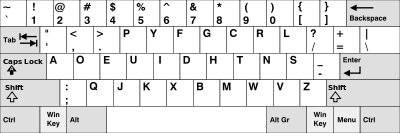
\includegraphics[width=\textwidth]{img/dvorak.png}
    \caption{Dvorak}
    \label{fig:dvorak}
  \end{minipage}
  \hfill
  \begin{minipage}[b]{0.45\textwidth}
    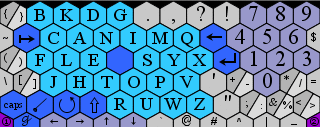
\includegraphics[width=\textwidth]{img/atomik.png}
    \caption{ATOMIK}
    \label{fig:atomik}
  \end{minipage}
\end{figure}

\begin{figure}[htb]
  \centering
  \begin{minipage}[b]{0.45\textwidth}
    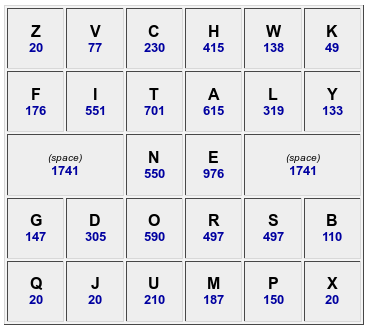
\includegraphics[width=\textwidth]{img/fitaly.png}
    \caption{FITALY}
    \label{fig:fitaly}
  \end{minipage}
  \hfill
  \begin{minipage}[b]{0.45\textwidth}
    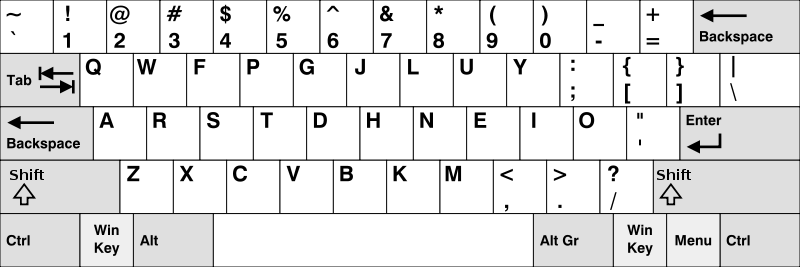
\includegraphics[width=\textwidth]{img/colemak.png}
    \caption{Colemak}
    \label{fig:colemak}
  \end{minipage}
\end{figure}

\chapter{Oblikovanje alternativne tipkovnice}
Ovo poglavlje obuhvaća opis samog problema te pristup njegovog rješavanja. Cilj ovog rada jest osmisliti alternativnu tipkovnicu za zaslone osjetljive na dodir koristeći Fittsov zakon. Jednostavnije rečeno, cilj je dizajnirati tipkovnicu s određenim rasporedom tipki koja bi korisniku omogućila brže unošenje teksta u odnosu na QWERTY tipkovnicu. Algoritam koji se koristi temelji se na zasadama Fittsovog zakona (detaljnije opisan u poglavlju \ref{sec:fitts}). Taj zakon predviđa vrijeme potrebno da korisnik reagira i pomakne \emph{nešto} s jedne lokacije na drugu. To \emph{nešto} može biti npr. kursor miša, ruka, noga ili konkretno što se tiče ovog rada: prst. To vrijeme je funkcija udaljenosti do odredišne lokacije i širine te lokacije: $f(D,W)$. U okviru pronalaženja optimalnog rasporeda znakova na tipkovnici, udaljenost predstavlja međusobnu udaljenost dvije tipke na tipkovnici koje će se uzastopno stisnuti, a širina jest širina same tipke. Kao što se već da naslutiti, cilj je minimizirati funkciju vremena što istovremeno znači i minimizirati vrijeme potrebno da se unese određeni tekst. Uzmimo kao primjer riječ PAS i da korisnik tekst unosi prstom jedne ruke. Kako bi se izračunalo vrijeme koje je potrebno da korisnik to unese treba izračunati udaljenost od P do A $d(P,A)$ i širinu od A $w(A)$, pa udaljenost od A do S $d(A,S)$ i širinu od S $w(S)$. Pretpostavlja se da je početni položaj korisnikova prsta iznad slova P, kada njega stisne potrebno je preći udaljenost $d(P,A)$ da bi se stisnula tipka A širine $w(A)$ pa udaljenost $d(A,S)$ da bi se stisnula tipka S širine $w(S)$. Iz ovoga se vidi kako će se pomoću Fittsovog zakona dobiti tipkovnica koja će imati slova koja se često uzastopno koriste, jedan blizu drugoga. Zbog toga je potrebno analizirati statistiku bigrama za ciljani jezik tipkovnice.

Kako bi se pronašao raspored tipki koji će prema Fittsovom zakonu imati najkraće vrijeme unosa teksta bilo bi najjednostavnije isprobati svaku moguću i pronaći onu s najmanjim vremenom. Ali to nije izvedivo, ako se uzme u obzir hrvatska abeceda koja ima 30 slova, potrebno je ispitati $30! = 2.65*10^{32}$ mogućih različitih razmještaja (starost svemira je $10^{10}$ sekundi). Ovaj problem predstavlja tipičan problem optimizacije, pitanje je kako pronaći minimum funkcije zadane Fittsovim zakonom uzevši u obzir sve moguće razmještaje slova. Postoje razne metode za rješiti taj problem. U ovom radu se koristio genetski algoritam. Genetski algoritam i način na koji je iskorišten detaljno je opisan u poglavlju \ref{sec:genetski}.

\section{Fittsov zakon}
\label{sec:fitts}
Fittsov zakon je opisni model ljudskog pokreta koji se primarno koristi u \emph{HCI-u}\footnote{Interakcija čovjeka i računala.} i \emph{ergonomiji}\footnote{Znanstvena disciplina koja istražuje ljudski organizam i ponašanje, te pruža podatke o prilagođenošću predmeta s kojima čovjek dolazi u kontakt.}. Kao što je već navedeno, Fittsov zakon predviđa vrijeme brzog pokreta do odredišne lokacije, to je funkcija udaljenosti do odredišta i širine tog odredišta. Ovaj zakon modelira čin pokazivanja (engl. \emph{act of pointing}), to može biti fizičko dodirivanje nekog objekta, primjerice rukom i prstom, a može biti i virtualno kao što je strelicom miša na računalu. Fittsov zakon se pokazao učinkovit u mnogo različitih slučajeva, koristeći razne dijelove tijela (ruke, noge, usne, kretanje oka...), u raznim okolinama (čak i pod vodom) i u raznim društvenim skupinama (mladi, stariji, ljudi s posebnim potrebama...). 

Ideja Fittsovog zakona prikazana je na slici \ref{fig:fitts} gdje se kao udaljenost do odredišta gleda udaljenost od dvije istaknute lokacije, a širina odredišta je širina "Take the Tour" gumba. Na slici \ref{fig:scroll} vidi se razlika između klizne trake (engl. \emph{scroll-bar}) kod OSX-a i Windows-a. Kod Windows-a su strelice za pomicanje klizne trake krajnje lijevo i krajnje desno, što više prati mentalni model osobe kojoj je to intuitivnije. S druge strane kod OSX-a su obe strelice jednu uz drugu kako bi se smanjilo vrijeme pomicanja strelice miša s jedne na drugu, što je konkretno ono čega se Fittsov zakon dotiče.

Paul Fitts je 1954. godine predložio metriku pomoću koje se vrednuje težina zadatka pokazivanja (brzog pomicanja na odredišnu lokaciju). Ta metrika se temelji na informacijskoj analogiji, gdje je $D$ udaljenost do odredišta i gleda se na njega kao na signal, a $W$ je širina ili tolerancija koja se ponaša kao šum. $ID$ predstavlja indeks težine (engl. \emph{index of difficulty}) i mjeri se u bitovima. Formula je dana izrazom \ref{eq:fitts}.
\begin{equation}
\label{eq:fitts}
ID = log_2(2D/W)
\end{equation}

Fitts je također predložio indeks izvedbe (engl. \emph{index of performance}) kao mjerilo ljudske izvedbe . Ova metrika kombinira $ID$ (\emph{index of difficulty}) s vremenom pomicanja $MT$ (\emph{movement time}) na odredišnu lokaciju. Prosječna stopa informacije koja je dobivena serijom pokreta jest prosječna informacija po pomicanju podijeljena s vremenom pomicanja. Formula je dana izrazom \ref{eq:fitts2}.
\begin{equation}
\label{eq:fitts2}
IP = ID/MT
\end{equation}
$MT$ je definiran izrazom \ref{eq:fitts3}. Parametri $a$ i $b$ koji najviše odgovaraju tom izrazu pronalaze se linearnom regresijom.
\begin{equation}
\label{eq:fitts3}
MT = a+b*ID = a+b*log_2(2D/W)
\end{equation}

\begin{figure}[htb]
  \centering
  \begin{minipage}[b]{0.45\textwidth}
    
\includegraphics[width=\textwidth]{img/fitts.png}
    \caption{Uporaba Fittsovog zakona}
    \label{fig:fitts}
  \end{minipage}
  \hfill
  \begin{minipage}[b]{0.45\textwidth}
    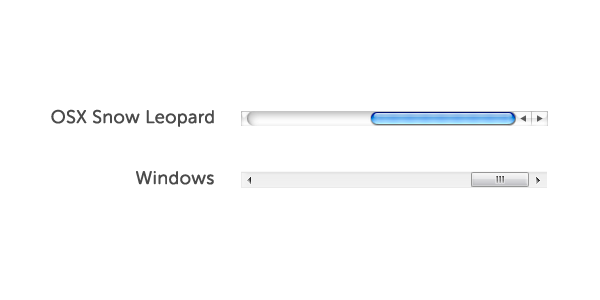
\includegraphics[width=\textwidth]{img/scroll.png}
    \caption{Uporaba Fittsovog zakona}
    \label{fig:scroll}
  \end{minipage}
\end{figure}


\subsection{Vrednovanje razmještaja tipki}
Za potrebe ovog rada korištena je modifikacija Fittsovog zakona kako bi se evaluirala pojedina tipkovnica. Formula je dana izrazom \ref{eq:fitts4}
\begin{equation}
\label{eq:fitts4}
t = \sum_{i=1}^{N}\sum_{j=1}^{N}\frac{P_{i,j}}{IP}log_2(\frac{D_{i,j}}{W_{i,j}} + 1)
\end{equation}
gdje je:
\begin{itemize}
\item $t$: prosječna vremenska cijena (engl. \emph{time cost})
\item $P$: matrica vjerojatnosti prelaska s jednog slova na drugu (bigrami)
\item $D$: matrica međusobne udaljenosti dva slova na tipkovnici
\item $W$: širina tipke na kojoj se nalazi određeno slovo
\item $IP$: Fittsov indeks izvedbe mjeren u bitovima po sekundi [$bit/s$]
\item $N$: broj slova u ciljanoj abecedi
\end{itemize}
Ovaj model se može pojednostavniti ako postavimo $W=IP=1$ što neće utjecati na konačne rezultate.

U nastavku je opisano što izraz \ref{eq:fitts4} zapravo znači. Kao primjer uzeta je tipkovnica prikazana na slici \ref{fig:fitts_primjer}. Prvo što treba je matrica vjerojatnosti $P$. Ona je dimenzija $N$x$N$ i izgleda različito za svaki jezik (za engleski jezik najveću će vrijednost imati polje koje označava bigram \emph{TH}). Nakon toga potrebno je izračunati matricu $D$. Udaljenost dva slova na tipkovnici se jednostavno računaju tako da se tipkovnica gleda kao šahovska ploča gdje svako slovo ima svoje koordinate. Primjerice udaljenost slova \emph{z} i \emph{d} je $1$, a udaljenost slova \emph{ć} i \emph{h} je $\sqrt{2^2+1^2} = 2.236$. Kada se izračunate vrijednosti provuku kroz izraz \ref{eq:fitts4} dobit će se vremensku cijena tipkovnice koja približno iznosi $1.038$. Jedinica ove vrijednosti nije bitna, bitno je jedino da postoji kriterij za usporedbu dvije tipkovnice. Što je vremenska cijena tipkovnice manja to je tipkovnica "bolja". Ovaj model preuzet je iz rada \emph{"Optimizing stylus keyboard layouts with a genetic algorithm: customization and internationalization" - Chad R. Brewbaker}.

Ovakva tipkovnica namijenjena je za unošenje teksta koristeći stilus ili jednim prstom. Kako bi se generirala tipkovnicu koja je idealnija za korištenje dva prsta (primjerice palčevima kao što to većina ljudi radi na pametnim uređajima) napravljene su neke izmjene u odnosu na prethodno opisani model. Svaka tipkovnica podijeljena je na dva dijela (lijevi i desni) od kojih je svaki dio namijenjen za lijevu, odnosno desnu ruku. Svaki dio ima svoje središte za koje se pretpostavlja da je lokacija iznad koje korisnik drži prst kada unosi tekst. Vremenska cijena ovakve tipkovnice računa se na malo drugačiji način. Uzmimo za primjer tipkovnicu na slici \ref{fig:fitts_primjer2}. Lijevo i desno središte označeni su crvenim kružićem. Znakovi \emph{B} i \emph{H} su na istoj strani (lijevoj) pa se pretpostavlja da će ih korisnik oba unijeti koristeći palac lijeve ruke. Njihova udaljenost se tada računa kao i prije te iznosi $2$. Znakovi \emph{R} i \emph{O} nalaze se na suprotnim stranama. Za njihovu udaljenost uzima se zbroj udaljenosti od lijevog središta do znaka \emph{R} i udaljenosti od desnog središta do znaka \emph{O}. Ovakav način računanja odabran je zbog toga što većina ljudi tako unosi tekst na pametnim uređajima. Kako bi se provjerila valjanost ovog modela napravljen je eksperiment koji je opisan u poglavlju 3.

\begin{figure}[htb]
  \centering
  \begin{minipage}[b]{0.48\textwidth}
    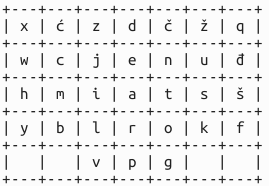
\includegraphics[width=\textwidth]{img/primjer.png}
    \caption{Primjer tipkovnice}
    \label{fig:fitts_primjer}
  \end{minipage}
  \hfill
  \begin{minipage}[b]{0.48\textwidth}
    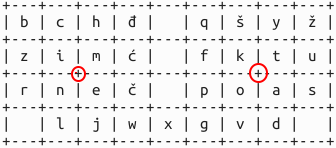
\includegraphics[width=\textwidth]{img/2hand_primjer.png}
    \caption{Primjer tipkovnice}
    \label{fig:fitts_primjer2}
  \end{minipage}
\end{figure}

\section{Genetski algoritam}
\label{sec:genetski}
Genetski ili genetički algoritam (GA)  je heuristička metoda optimiranja koja imitira prirodni evolucijski proces. Evolucija je robustan proces pretraživanja prostora rješenja. Živa bića se tijekom evolucije prilagođavaju uvjetima u prirodi, tj. životnoj okolini. Analogija evolucije kao prirodnog procesa i genetskog algoritma kao metode optimiranja, očituje se u procesu selekcije i genetskim operatorima. Mehanizam odabira nad nekom vrstom živih bića u evolucijskom procesu čine okolina i uvjeti u prirodi. U genetskim algoritmima ključ selekcije je funkcija cilja, koja na odgovarajući način predstavlja problem koji se rješava. Slično kao što su okolina i uvjeti u prirodi ključ selekcije nad nekom vrstom živih bića, tako je i funkcija cilja ključ selekcije nad populacijom rješenja u genetskom algoritmu. Naime, u prirodi jedinka koja je najbolje prilagođena uvjetima i okolini u kojoj živi ima najveću vjerojatnost preživljavanja i parenja, a time i prenošenja svojega genetskog materijala na svoje potomke. Za genetski algoritam jedno rješenje je jedna jedinka. Selekcijom se odabiru dobre jedinke koje se prenose u slijedeću populaciju, a manipulacijom genetskog materijala stvaraju se nove jedinke. Takav ciklus selekcije, reprodukcije i manipulacije genetskim materijalom jedinki ponavlja se sve dok nije zadovoljen uvjet zaustavljanja evolucijskog procesa. Konačan rezultat je populacija jedinki (potencijalnih rješenja). Najbolja jedinka u zadnjoj iteraciji predstavlja rješenje optimiranja. Genetski algoritam izvršava se uporabom operatora križanja, mutacije, selekcije i reprodukcije. Svaki od njih objašnjen je u nastavku.

\subsection{Operator križanja}
U procesu križanja (engl. \emph{crossover}) sudjeluju dvije jedinke koje se nazivaju \emph{roditelji}. Dakle, križanje je binarni operator. Križanjem nastaju jedna ili dvije nove jedinke koje se nazivaju \emph{djeca}. Najvažnija karakteristika križanja jest da \emph{djeca} nasljeđuju svojstva svojih roditelja. Ako su roditelji \emph{dobri} (prošli su proces selekcije), tada će najvjerojatnije i \emph{dijete} biti dobro, ako ne i bolje od svojih roditelja. Ako se jedinka predstavi kao niz bitova onda se križanje implementira slično kao što je prikazano na slici \ref{fig:krizanje}. Bitno je napomenuti da se križanje može izvesti na mnogo različitih načina, ovisno o problemu i načinu prikaza jedinke.

\begin{figure}[htb]
\centering
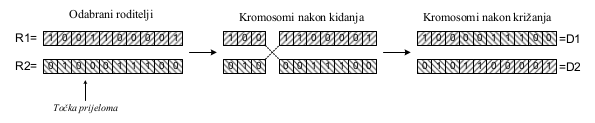
\includegraphics[width=12cm]{img/krizanje.png}
\caption{Križanje s jednom točkom prijeloma}
\label{fig:krizanje}
\end{figure}

\subsection{Operator mutacije}
Mutacija ili slučajna promjena jednog ili više gena je unarni operator koji djeluje nad jednom jedinkom. Rezultat mutacije je izmijenjena jedinka. Parametar koji određuje vjerojatnost mutacije $p_m$ jednog bita je ujedno i parametar algoritma. Ako vjerojatnost mutacije teži k jedinici, tada se algoritam pretvara u algoritam slučajne pretrage prostora rješenja. S druge strane, ako vjerojatnost mutacije teži k nuli, postupak će najvjerojatnije već u početku optimiranja stati u nekom lokalnom optimumu. \emph{Jednostavna mutacija} svaki bit kromosoma mijenja s jednakom vjerojatnošću $p_m$.

\begin{figure}[htb]
\centering
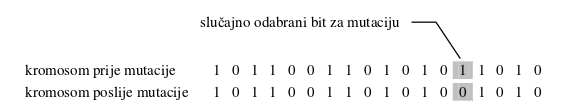
\includegraphics[width=12cm]{img/mutacija.png}
\caption{Jednostavna mutacija}
\label{fig:mutacija}
\end{figure}

\subsection{Operator selekcije}
Jedan od centralnih mehanizama, kako kod većine populacijskih algoritama pa i općenito, jest mehanizam \emph{selekcije}. Kod populacijskih algoritama zadaća operatora selekcije jest osigurati mehanizam koji će češće boljim rješenjima dati priliku da sudjeluju u produkciji novih rješenja, čime će se proces pretraživanja prostora rješenja voditi u područja koja više obećavaju. Postoji više različitih vrsta selekcija.

\emph{Proporcionalna selekcija} (engl. \emph{Roulette-wheel selection} funkcionira na način da sve jedinke postavimo na kolo, tako da bolja jedinka ima veću površinu na kolu (prikazano na slici \ref{fig:selekcija}). Potom zavrtimo kolo i pogledamo na kojoj se jedinki kolo zaustavilo. S obzirom da jedinki pripada to veći dio oboda kola što ima veću dobrotu, ponavljamo li eksperiment puno puta, bolje jedinke će biti češće birane od lošijih, i ta će vjerojatnost biti upravo proporionalna dobroti same jedinke.

\begin{figure}[htb]
\centering
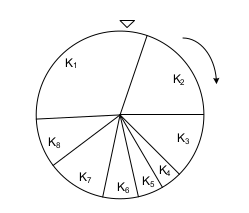
\includegraphics[width=6cm]{img/selekcija.png}
\caption{Proporcionalna selekcija}
\label{fig:selekcija}
\end{figure}

Kod \emph{k-turnirske selekcije} se iz populacije posredstvom slučajnog mehanizma odabire \emph{k} jedinki, i potom uzima najbolju. Ukoliko trebamo \emph{n} roditelja,, naprosto ćemo \emph{n} puta ponoviti turnirsku selekciju.

\subsection{Operator reprodukcije}
Reprodukcijom se jednostavno jedinka prenosi iz jedne generacije u drugu. Ta jedinka se odabere operatorom selekcije.

\begin{algorithm}
\caption{Genetski algoritam - pseudokod}
\label{alg:genetski}
\begin{algorithmic}
\STATE{P = stvoriPocetnuPopulaciju(VELICINA)}
\STATE{evaluiraj(P)}
\REPEAT
\STATE{novaPopulacija P' = $\emptyset$}
\WHILE{velicina(P') < VELICINA}
\STATE{odaberi R1 i R2 iz P}
\STATE{\{D1, D2\} = krizaj(R1, R2)}
\STATE{mutiraj D1, mutiraj D2}
\STATE{dodaj D1 i D2 u P'}
\ENDWHILE
\STATE{P = P'}
\UNTIL{uvjetZadovoljen}
\end{algorithmic}
\end{algorithm}

\begin{figure}[htb]
\centering
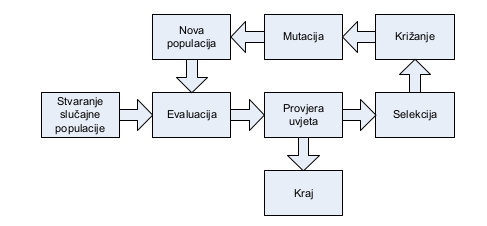
\includegraphics[width=12cm]{img/genetski_shema.png}
\caption{Shema genetskog algoritma}
\label{fig:genetski_shema}
\end{figure}

\subsection{Primjena genetskog algoritma}
Jedinku u genetskom algoritmu predstavlja jedna tipkovnica sa svojim oblikom i rasporedom tipki. Jedna generacija sadrži $500$ jedinki, a $1000$ je postavljen za maksimalan broj generacija (uvjet zaustavljanja algoritma). Algoritam koristi operatore križanja, selekcije, mutacije i reprodukcije kako bi pronašao optimalno rješenje. Tip selekcije koji se koristio jest \emph{k-turnirska selekcija} gdje je \emph{k} postavljen na $24$. Mutacija je implementirana na način da su slučajnom odabirom zamijenjene pozicije od $p\%$ znakova na tipkovnici. $p$ je postavljen na $0.3$. Križanje je napravljeno tako da su svi znakovi s pojedine tipkovnice po redu nanizani u polje. Točka prekida polja je središnji element. Nakon prekida dvije polovice se zamijene i tada nastaju 2 nova polja. Svako polje može sadržavati duple znakove. Taj problem je rješen tako da su u svakom pronađeni znakovi koji nedostaju i stavljeni umjesto duplikata. Proces križanja prikazan je na slici \ref{fig:krizanje_primjer}. \\TODO opisat detaljnije ? 

\begin{figure}[htb]
\centering
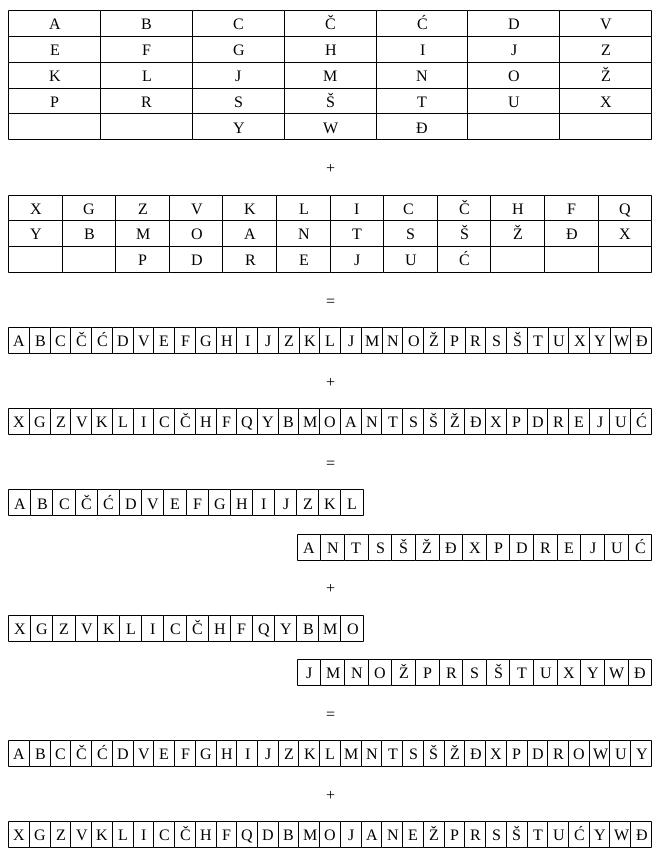
\includegraphics[width=16cm]{img/krizanje_tip.png}
\caption{Primjer križanja tipkovnica}
\label{fig:krizanje_primjer}
\end{figure}

\clearpage

\section{Rješenja genetskog algoritma}
U ovom poglavlju će biti predstavljene najbolje tipkovnice koje su dobivene genetskim algoritmom te način njihove implementacije. Isprobano je nekoliko različith izgleda (engl. \emph{layout}) tipkovnica za korištenje pomoću jednog i pomoću dva prsta. Neke od njih prikazane su na sljedećim slikama //TODO ref bla bla

Moguće je da postoje i neki izgledi koji bi se pokazali optimalniji prema Fittsovom zakonu ali zbog ograničenosti vremena testirani su samo pojedini. Tipkovnica namijenjena korištenju s jednim prstom prikazana je na slici \ref{fig:FuryKey1} i prema Fittsovom zakonu njena vremenska cijena iznosi $1.038$. Može se lako uočiti da se sva često korištena slova u hrvatskom jeziku nalaze u sredini dok se ona rijeđe korištena nalaze na rubovima. Takav razmještaj omogućuje brže unošenje teksta. Tipkovnica namijenjena korištenju s dva prsta prikazana je na slici \ref{fig:FuryKey2} i njena vremenska cijena iznosi $0.948$. Prema tome tipkovnica \emph{FuryKey2} se pokazala učinkovitijom za korištenje što je i logično jer se koristeći dva prsta tekst može brže unositi nego s jednim. Kako bi se provjerilo imaju li navedeni rezultati smisla i je li \emph{FuryKey1} zaista bolje koristiti s jednim prstom, a \emph{FuryKey2} s dva prsta, potrebno je provesti eksperiment pomoću kojeg će se nad grupom ispitanika evaluirati obe tipkovnice. Provedeni eksperiment je opisan u poglavlju \ref{ch:eksperiment}.

\begin{figure}[htb]
  \centering
  \begin{minipage}[b]{0.48\textwidth}
    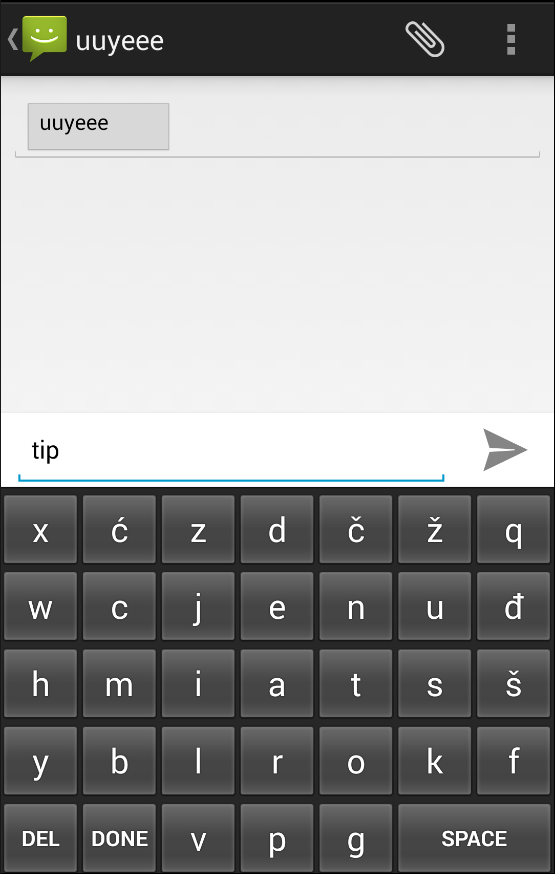
\includegraphics[width=\textwidth]{img/FuryKey1.PNG}
    \caption{FuryKey1 - tipkovnica namijenjena za tipkanje jednim prstom ili stilusom}
    \label{fig:FuryKey1}
  \end{minipage}
  \hfill
  \begin{minipage}[b]{0.48\textwidth}
    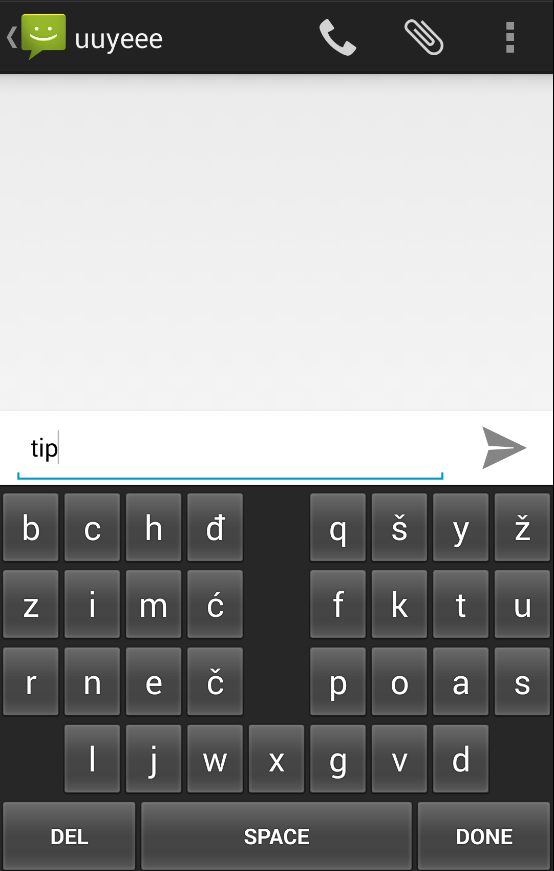
\includegraphics[width=\textwidth]{img/FuryKey2.PNG}
    \caption{FuryKey2 - tipkovnica namijenjena za tipkanje s dva prsta}
    \label{fig:FuryKey2}
  \end{minipage}
\end{figure}

\subsection{Implementacija tipkovnica za Android operacijski sustav}
Obe tipkovnice implementirane su za pametne uređaje s \emph{Android} operacijskim sustavom. //TODO napisat što je to Android ? napisat ponešto o soft keyboardima i način implementacije soft keyboarda ? (pitat mentora)

\chapter{Provedba eksperimenta i obrada rezultata}
\label{ch:eksperiment}
TODO napisat nešto općenito o eksperimentima i njihovoj važnosti
\section{Oblikovanje eksperimenta}
TODO nešto dodat, opisat što su to nezavisne, zavisne varijable itd...
bacit oko na mackenzievu knjigu\\
Ako se svako mjerenje ponavlja za svakog ispitanika onda je oblik eksperimenta \emph{unutar sudionika} (engl. \emph{within-subjects}). Svi ispitanici tada imaju potpuno jednake uvjete pri provedbi eksperimenta. Kod \emph{između sudionika} (engl. \emph{between-subjects}) oblika ispitanici se dijele na više grupa i svaka grupa dobija drugačije uvjete ispitivanja dok unutar jedne grupe ispitanici imaju iste uvjete ispitivanja. Načelno, kod \emph{između sudionika} oblikovanja potrebno je više ispitanika da bi se proveo isti broj mjerenja,a kod \emph{unutar sudionika} potrebno je provesti više testiranja na pojedinom ispitaniku. Ponekad eksperiment mora biti \emph{između sudionika} ako npr. promatramo učinak ljevorukih i desnorukih ispitanika na određenom testu. Ponekad mora biti \emph{unutar sudionika} ako se npr. promatra stjecanje iskustva kod pojedinog ispitanika. Prednost \emph{unutar sudionika} je njegova jednostavnost, nije potrebno uravnotežavati grupe jer postoji samo jedna, dok se kod \emph{između sudionika} potrebno pobrinuti da grupe budu više-manje jednake. To se najčešće radi tako da se ispitanici nasumično odaberu za svaku grupu. Prednost \emph{između sudionika} je to što se smanjuje utjecaj između uvjeta ispitivanja. Do toga dolazi kada ispitanik prelazi s jednog testa na drugi, u tom procesu na drugi test prenosi iskustva i znanje koje je stekao u prethodnom.

Kao što je već navedeno, kad se koristi \emph{unutar sudionika} oblik eksperimenta, svakog ispitanika se testira na svakom testu te se zbog toga učinak ispitanika svakim testom može poboljšati ili čak pogoršati u nekim slučajevima. To je razlog radi kojeg se ponekad, u testovima nakon prvog, ne dobivaju stvarni rezultati. Da bi se to popravilo koristi se metoda suprotstavljanja i latinski kvadrati. Svaki ispitanik dobija testove u drugačijem poretku. Slika \ref{fig:latinski_kvadrat} predstavlja latinski kvadrat reda $3$. Svako slovo predstavlja test koji ispitanik izvršava. U ovom slučaju svi bi ispitanici bili podijeljeni u 3 grupe i svaki bi redak odgovarao redoslijedu kojim bi pojedina grupa radila zadane testove.

\begin{figure}[htb]
\centering
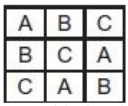
\includegraphics[width=4cm]{img/latinski_kvadrat.png}
\caption{Latinski kvadrat reda 3}
\label{fig:latinski_kvadrat}
\end{figure}

\section{Eksperimentalno vrednovanje tipkovnica}
Cilj eksperimenta je vrednovati prethodno opisane tipkovnice \emph{FuryKey1} i \emph{FuryKey2} te ih usporediti s QWERTZ tipkovnicom. Nadalje, potrebno je ispitati na koji je način najbolje koristiti svaku od navedenih tipkovnica (horizontalno ili vertikalno, tipkanje s jednim ili dva prsta). Provedeni eksperiment oblikovan je na sljedeći način:
\\\\\textbf{Varijable eksperimenta}
\begin{itemize}
\item Nezavisne varijable:
\begin{itemize}
\item tipkovnica: FuryKey1, FuryKey2, QWERTZ
\item veličina pametnog uređaja: 7", 10"
\item način korištenja: jedan prst, dva prsta
\item položaj pametnog uređaja: horizontalno \engl{landscape}, vertikaln \engl{portrait}
\end{itemize}
\item Zavisne varijable:
\begin{itemize}
\item brzina unošenja teksta: broj riječi koje ispitanik prosječno unese u jednoj minuti, mjerna jedinica je stoga $wpm$ \engl{words per minute}
\item broj pogrešaka ER \engl{error rate}: broj pogrešaka koje ispitanik napravi tijekom unosa teksta
\end{itemize}
\item Zbunjujuće varijable
\begin{itemize}
\item iskustvo: uzevši u obzir da će ispitanik jednu tipkovnicu koristiti više puta za redom, doći će do pojave učenja što nije dobro za eksperiment,zato se korisito latinski kvadrat da bi se smanjio učinak učenja
\end{itemize}
\end{itemize}

Eksperiment je oblikovan kao mješavina \emph{unutar sudionika} i \emph{između sudionika}. Osam ispitanika podijeljeno je u dvije grupe po četvero. Jedna je grupa koristila samo \emph{FuryKey1}, a druga samo \emph{FuryKey2}. Na taj način neće doći do nikakve međuovisnosti rezultata jedne i druge tipkovnice. Kako bi se smanjio učinak učenja napravljen je latinski kvadrat i prema njemu su svi ispitanici u jednoj grupi testirani različitim redoslijedom. On je prikazan na slici \ref{fig:lat} gdje slova \emph{H} i \emph{V} označavaju položaj pametnog uređaja (horizontalno, vertikalno), brojevi $1$ i $2$ označavaju broj prstiju koji se koristi pri unošenju teksta. Svi ispitanici su unosili 2 različita bloka teksta za svaki način korištenja.

\begin{figure}[htb]
\centering
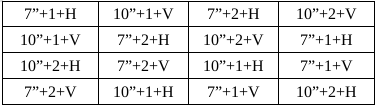
\includegraphics[width=10cm]{img/lat.png}
\caption{Latinski kvadrat reda 4}
\label{fig:lat}
\end{figure}

\subsection{Prikaz i interpretacija rezultata}
Mjerna jedinica svih prikazanih rezultata je $wpm$. Rezultati su dobiveni prema izrazu \ref{eq:wpm} gdje $t$ predstavlja izmjereno vrijeme u sekundama, $n$ broj unešenih riječi, a $ER$ broj pogrešaka koje je korisnik pri unosu načinio.

\begin{equation}
\label{eq:wpm}
wpm = \frac{60(n-ER)}{t}
\end{equation}
Tablica \ref{tab:furykey1_sve} predstavlja sve dobivene rezultate za \emph{FuryKey1}, tablica \ref{tab:furykey2_sve} za \emph{FuryKey2} dok su na tablicama \ref{tab:furykey1_avg} i \ref{tab:furykey2_avg} prikazani prosječni rezultati za oba bloka teksta. Tablica \ref{tab:qwertz_sve} prikazuje rezultate dobivene pri testiranju QWERTZ tipkovnice.
Na slikama \ref{chart:furykey1_sve_graf} i \ref{chart:furykey2_sve_graf} grafički su prikazani rezultati iz prethodnih tablica. Kod oba grafa se može lako uočiti povećanje brzine pri unošenju drugog bloka teksta. Graf \ref{chart:usporedba} prikazuje usporedbu svih testiranih tipkovnica. Iz grafa se vidi kako se QWERTZ pokazao dosta učinkovitiji, ali to je i očekivano. Nadalje, može se vidjeti kako se kod nekih načina unošenja teksta boljom pokazala \emph{FuryKey1}, a kod nekih \emph{FuryKey2}. Te rezultate potrebno je još detaljnije ispitati. Na grafovima \ref{chart:furykey1_HV} i \ref{chart:furykey2_HV} prikazana je usporedba horizontalnog i vertikalnog načina držanja za obe tipkovnice. Vidi se kako je kod obe tipkovnice učinkovitiji vertikalni način. To je zbog toga što je tada međusobna udaljenost tipki manja nego kod horizontalnog načina. Grafovi \ref{chart:furykey1_12} i \ref{chart:furykey2_12} prikazuju usporedbu tipkanja s jednim i dva prsta. Tipkovnica \emph{FuryKey1} namijenjena je za korištenje s jednim prstom, a \emph{FuryKey2} za korištenje s dva prsta. To su rezultati i potvrdili. Konačno, graf \ref{chart:uk} prikazuje ukupnu usporedbu obe tipkovnice (cjelokupni prosjek svih položaja i načina unošenja pametnog uređaja). Rezultati eksperimenta pokazuju da je \emph{FuryKey2} učinkovitija.

Bitno je napomenuti da su za provedbu eksperimenta tipkovnice testirane nad \emph{samo} 8 ispitanika. Zbog toga ovi podatci ne mogu biti stvarni pokazatelj učinkovitosti testiranih tipkovnica. Potrebno je eksperiment provesti s mnogo više ispitanika, ali to nije napravljeno zbog ograničenosti resursa i vremena. Bez obzira na to, prikazani rezultati i način mjerenja služi kao model koji bi poslužio za provođenje eksperimenta većeg razmjera.

\begin{figure}[htb]
\centering
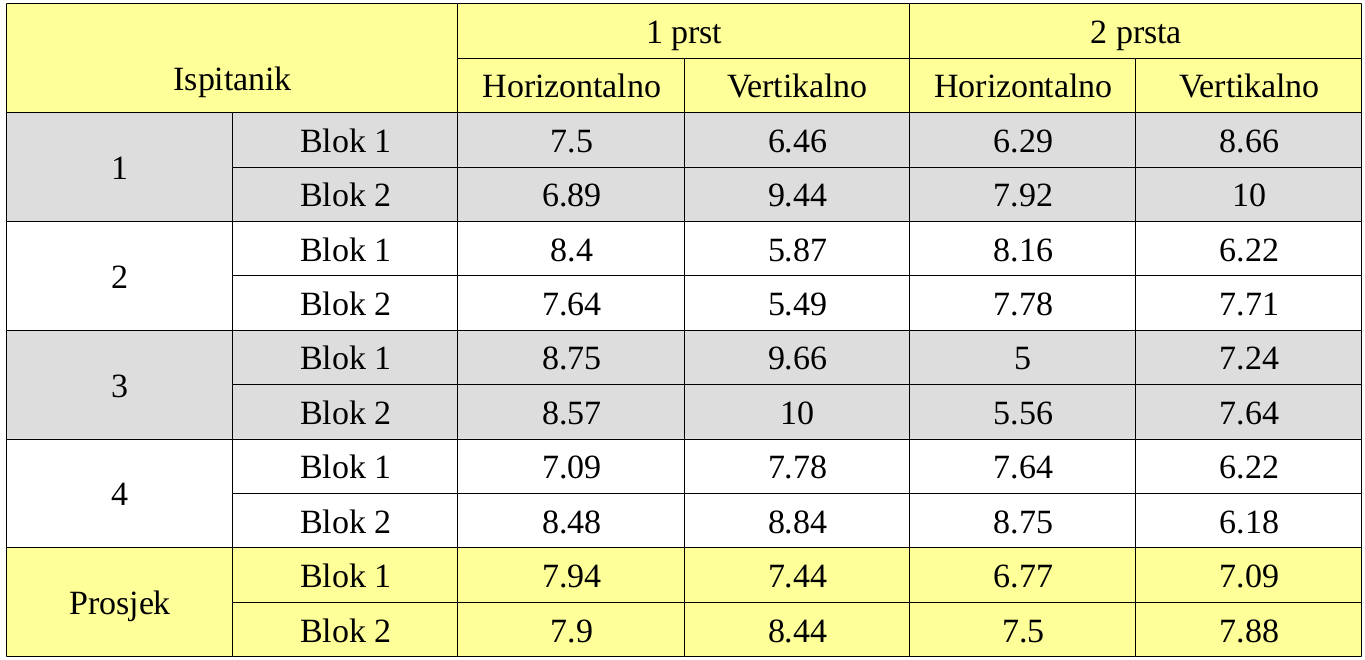
\includegraphics[width=14cm]{img/furykey1_sve.png}
\captionof{table}{Rezultati mjerenja za FuryKey1}
\label{tab:furykey1_sve}
\end{figure}

\begin{figure}[htb]
\centering
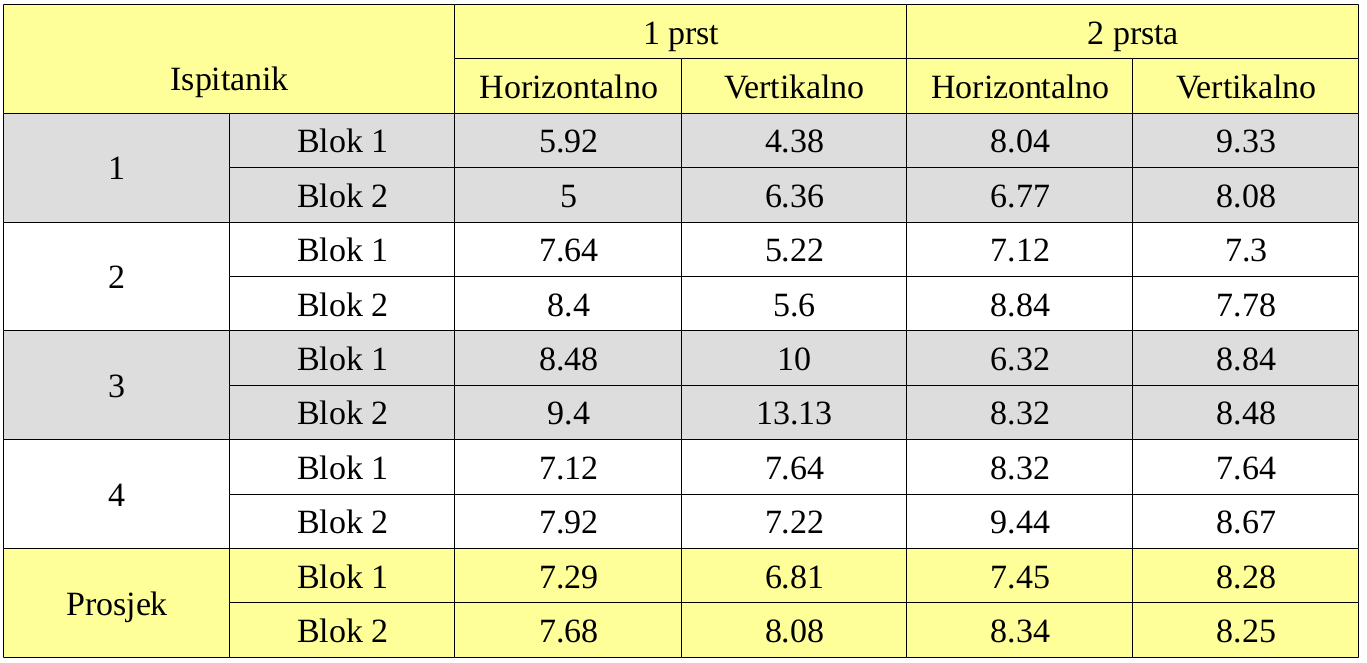
\includegraphics[width=14cm]{img/furykey2_sve.png}
\captionof{table}{Rezultati mjerenja za FuryKey2}
\label{tab:furykey2_sve}
\end{figure}

\begin{figure}[htb]
\centering
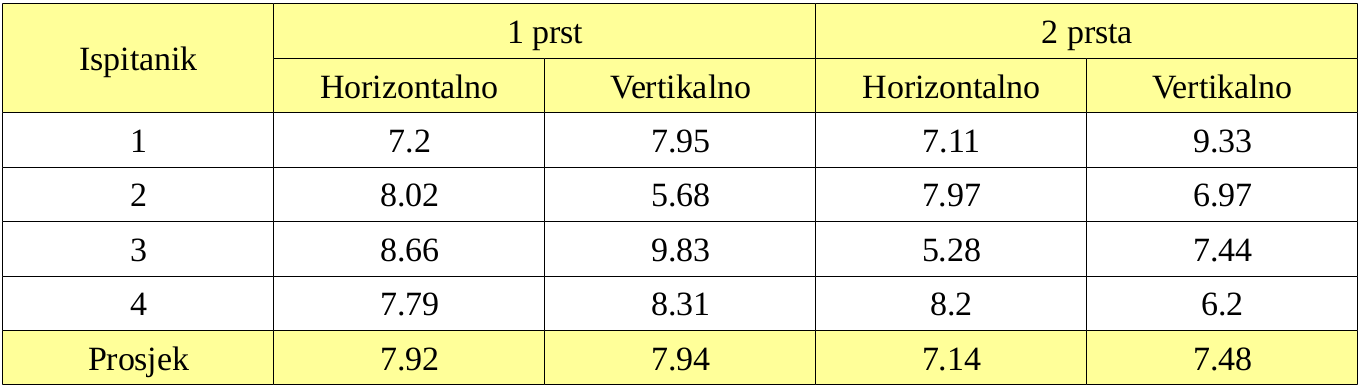
\includegraphics[width=14cm]{img/furykey1_prosjek.png}
\captionof{table}{Prosječni rezultati za FuryKey1}
\label{tab:furykey1_avg}
\end{figure}

\begin{figure}[htb]
\centering
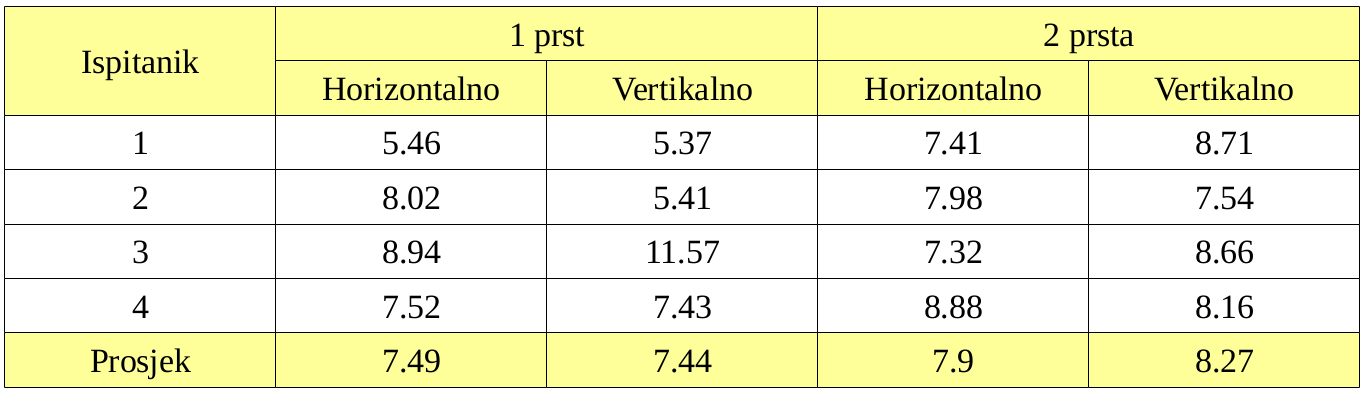
\includegraphics[width=14cm]{img/furykey2_prosjek.png}
\captionof{table}{Prosječni rezultati za FuryKey2}
\label{tab:furykey2_avg}
\end{figure}

\begin{figure}[htb]
\centering
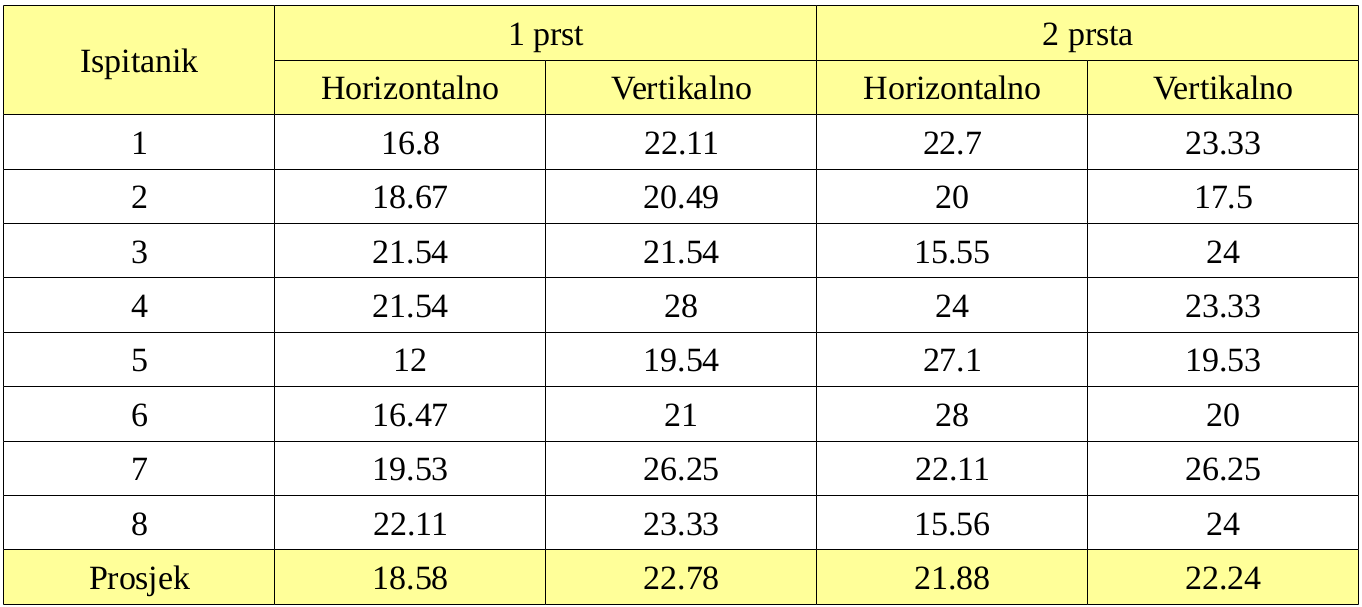
\includegraphics[width=14cm]{img/qwertz_sve.png}
\captionof{table}{Rezultati mjerenja za QWERTZ}
\label{tab:qwertz_sve}
\end{figure}

\begin{figure}[htb]
\centering
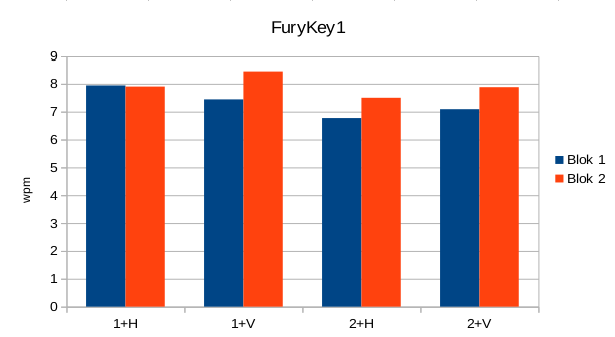
\includegraphics[width=14cm]{img/furykey1_sve_graf.png}
\caption{Grafički prikaz rezultata za FuryKey1}
\label{chart:furykey1_sve_graf}
\end{figure}

\begin{figure}[htb]
\centering
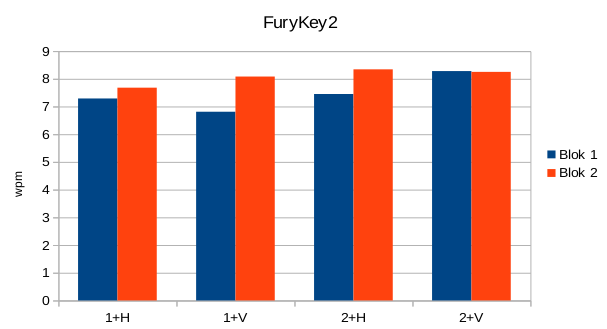
\includegraphics[width=14cm]{img/furykey2_sve_graf.png}
\caption{Grafički prikaz rezultata za FuryKey2}
\label{chart:furykey2_sve_graf}
\end{figure}

\begin{figure}[htb]
\centering
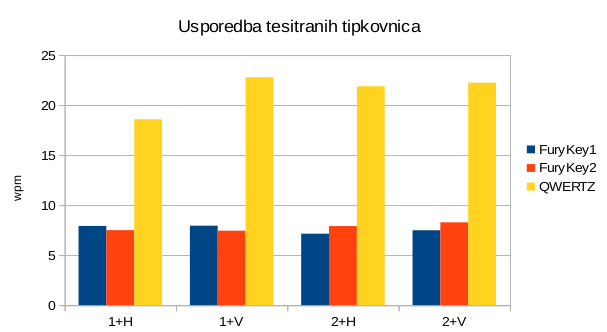
\includegraphics[width=14cm]{img/usporedba.png}
\caption{Usporedba FuryKey1, FuryKey2 i QWERTZ}
\label{chart:usporedba}
\end{figure}

\begin{figure}[htb]
\centering
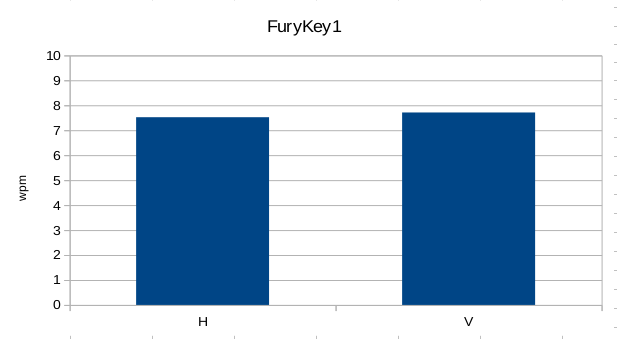
\includegraphics[width=14cm]{img/furykey1_HV.png}
\caption{Usporedba za horizontalni i vertikalni način držanja (H=7,52 V=7,71)}
\label{chart:furykey1_HV}
\end{figure}

\begin{figure}[htb]
\centering
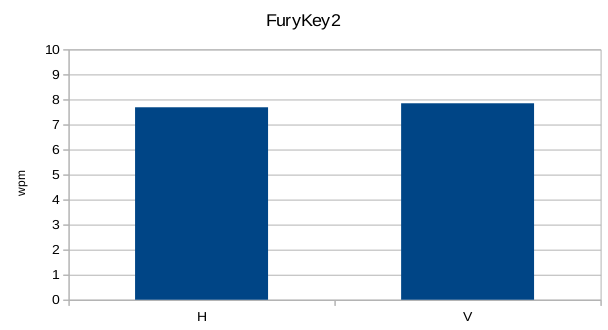
\includegraphics[width=14cm]{img/furykey2_HV.png}
\caption{Usporedba za horizontalni i vertikalni način držanja (H=7,69 V=7,85)}
\label{chart:furykey2_HV}
\end{figure}

\begin{figure}[htb]
\centering
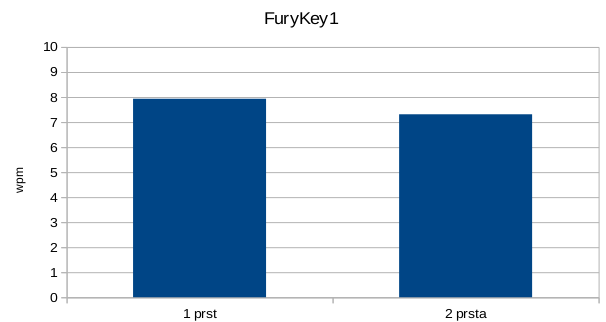
\includegraphics[width=14cm]{img/furykey1_12.png}
\caption{Usporedba za korištenje s jednim i s dva prsta (1 prst=7,93 2 prsta=7,31)}
\label{chart:furykey1_12}
\end{figure}

\begin{figure}[htb]
\centering
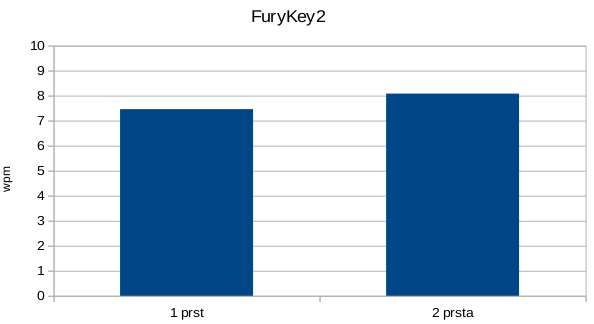
\includegraphics[width=14cm]{img/furykey2_12.png}
\caption{Usporedba za korištenje s jednim i s dva prsta (1 prst=7,46 2 prsta=8,08)}
\label{chart:furykey2_12}
\end{figure}

\begin{figure}[htb]
\centering
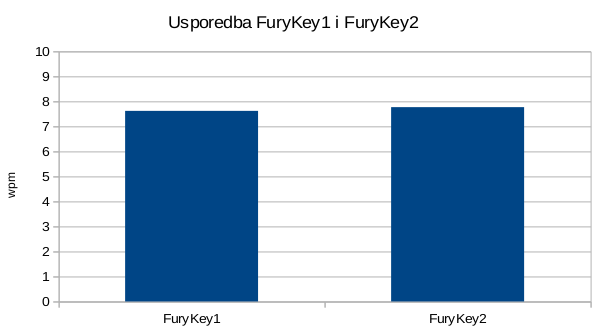
\includegraphics[width=14cm]{img/usporedba_ukupno.png}
\caption{Ukupna usporedba učinkovitosti (FuryKey1=7,62 FuryKey2=7,77)}
\label{chart:uk}
\end{figure}

\chapter{Zaključak}
Zaključak.

\bibliography{literatura}
\bibliographystyle{fer}

\begin{sazetak}
Sažetak na hrvatskom jeziku.

\kljucnerijeci{Ključne riječi, odvojene zarezima.}
\end{sazetak}

% TODO: Navedite naslov na engleskom jeziku.
\engtitle{Alternative Touchscreen Keyboard Based on Fitts Law}
\begin{abstract}
Abstract.	

\keywords{Keywords.}
\end{abstract}

\end{document}
